\chapter{Toric Hyperk{\"a}hler Manifolds}

\section{Hyperk{\"a}hler Reduction}

The quaternionic vector space $\HH^{N}$ is a flat \HK manifold with complex structures $J_{1}, J_{2}, J_{3}$ given by right multiplication by $i, j, k$ respectively. The real torus $T^{N}$ acts on $\HH^{N}$ by left diagonal multiplication and preserves the \HK structure. We may choose one complex structure, say $J_{2}$, and identify $\HH^{N}$ with $\CC^{N} \times \CC^{N}$, so that the action of $T^{N}$ can be written as
\begin{equation*}
	t\cdot (z,w) = (t\cdot z, t^{-1} \cdot w).
\end{equation*}
Alternatively, choosing the complex structure $J_{1}$ we may identify $\HH^{N}$ with the cotangent bundle $T^{\ast}\CC^{N}$, with the natural torus action induced from that on $\CC^{N}$.

The three moment maps $\m_{1}, \m_{2}, \m_{3}$ corresponding to the complex structures may be written as
\begin{equation*}
	\begin{split}
		\m_{1}(z,w) &= \frac{1}{2}\sum_{k=1}^{N}\big( |z_{k}|^{2} - |w_{k}|^{2} \big) e_{k} + c_{1},\\
		(\m_{2} + \sqrt{-1}\m_{3} )(z,w) &= \sum_{k=1}^{N}(z_{k}w_{k})e_{k} + c_{2} + \sqrt{-1}c_{3},
	\end{split}
\end{equation*}
for arbitrary constants $c_{1}, c_{2}, c_{3} \in \RR^{N}$, and where the $e_{k}$, $k = 1, \ldots, N$, are the standard basis vectors in $(\mf{t}^{N})^{\ast} \cong \RR^{N}$. Observe now that in this case, unlike in the Delzant construction previously used for toric manifolds, that the \HK moment map $\m = (\m_{1}, \m_{2}, \m_{3})$ is surjective onto $\RR^{3N}$.

Now let $u_{i} = \imath^{\ast}(e_{i})$, $i = 1,\ldots N$ define a subtorus $K$ of $T^{N}$ as $K = \ker(\pi)$, assuming like before that the vectors $u_{i}$ are $\ZZ$-valued, primitive, and generate $\RR^{n}$. The moment maps for the action of $K$ are
\begin{equation*}
\begin{split}
	\m_{1}(z,w) &= \frac{1}{2}\sum_{k=1}^{N}\big( |z_{k}|^{2} - |w_{k}|^{2} \big) \alpha_{k} + c_{1},\\
	(\m_{2} + \sqrt{-1}\m_{3} )(z,w) &= \sum_{k=1}^{N}(z_{k}w_{k})\alpha_{k} + c_{2} + \sqrt{-1}c_{3},
\end{split}
\end{equation*}
where $\alpha_{k} = \imath^{\ast}(e_{k})$, and where the constants $c_{j}$ are of the form
\begin{equation*}
	c_{j} = \sum_{k = 1}^{N}\lambda_{k}^{(j)}\alpha_{k},\qquad (j = 1,2,3),
\end{equation*}
for $\lambda_{k}^{(j)} \in \RR$. As in (ref BD), we shall adopt the notation
\begin{equation*}
	\lambda_{k} = (\lambda_{k}^{(1)}, \lambda_{k}^{(2)}, \lambda_{k}^{(3)} ),\quad (k = 1,\ldots, N),
\end{equation*}
and also denote the \HK quotient $\mu^{-1}(0)/K$ corresponding to $\underline{u} = (u_{1}, \ldots, u_{N})$ and $\underline{\lambda} = (\lambda_{1},\ldots, \lambda_{N})$ by $M(\underline{u}, \underline{\lambda})$, or even just by $M$.

The action on $T^{n} = T^{N}/K$ on $M(\underline{u}, \underline{\lambda})$ preserves the \HK structure and gives rise to another \HK moment map $\phi = (\phi_{1}, \phi_{2}, \phi_{3}): M(\underline{u}, \underline{\lambda}) \rightarrow (\mf{t}^{n})^{\ast} \otimes \RR^{3} \cong \RR^{3n}$. Finally, we will need to consider the following hyperplanes in $\RR^{n}$
\begin{equation*}
	H_{k}^{(j)} = \{ y \in \RR^{n} \st \langle y, u_{k} \rangle = \lambda_{k}^{(j)} \},\quad (j = 1,2,3,\quad k = 1,\ldots, N)
\end{equation*}
and the codimension 3 flats (affine subspaces) in $\RR^{3n}$
\begin{equation*}
	H_{k} = H_{k}^{(1)} \times H_{k}^{(2)} \times H_{k}^{(3)}.
\end{equation*}

\section{Hyperplane Arrangements}

It is the flats $H^{k}$ defined in the previous section that determine the corresponding \HK reduction, instead of the intersection of half-spaces as in the toric case. The following two theorems determine the necessary and sufficient conditions for the \HK quotient $\m^{-1}(0)/K$ to be either smooth or an orbifold respectively; their proofs can be found in (BD).

\begin{thm}
	Suppose we have primitive vectors $u_{1},\ldots u_{N} \in \ZZ^{n}$ that generate $\RR^{n}$, and elements $\lambda_{1}, \lambda_{2}, \lambda_{3} \in \RR^{3}$ such that the flats $H_{k}$ are distinct. Then the \HK quotient $M(\underline{u},\underline{\lambda})$ is smooth if and only if every $n+1$ flats among the $H_{k}$ have empty intersection, and whenever some $n$ flats $H_{k_{1}}, \ldots H_{k_{n}}$ have non-empty intersection, then the set $\{ u_{k_{1}}, \ldots, u_{k_{n}}  \}$ forms a $\ZZ$-basis for $\ZZ^{n}$.
\end{thm}

Let $\mf{t}^{N} \cong \RR^{N}$ and $\mf{t} \cong \RR^{n}$ be real vector spaces of dimensions $N$ and $n$ respectively, with integer lattices $\mf{t}_{\ZZ}^{N} \subset \mf{t}^{N}$ and $\mf{t}_{\ZZ}^{n} \subset \mf{t}^{n}$. Let $\{e_{1},\ldots, e_{N}  \}$ be an integer basis for $\mf{t}_{\ZZ}^{N}$ and $\{e^{1},\ldots, e^{N}\}$ be the respective dual basis for $(\mf{t}_{\ZZ}^{N})^{\ast}$. Now suppose that we are given $N$ non-zero integer vectors $\{u_{1},\ldots, u_{N}  \}$ that belong to $\mf{t}_{\ZZ}^{n}$, which space the space $\mf{t}^{n}$ over the real numbers $\RR$.

\section{The Core and Extended Core of a Hypertoric Variety}



\section{Symplectic Cutting}

Let $(M,\w)$ be a symplectic manifold with a Hamiltonian $S^{1}$-action whose moment map is $\Phi: M \rightarrow \RR$. Now consider the product $M \times \CC$ with the product symplectic structure and the $S^{1}$-action
\begin{equation*}
	e^{i\theta}\cdot[m,\xi] \longmapsto [ e^{i\theta}\cdot m, e^{-i\theta} \xi ],
\end{equation*}
and corresponding moment map
\begin{equation*}
	\Phi_{\text{cut}}[m, \xi] \longmapsto \Phi(m) - |\xi|^{2}.
\end{equation*}

The \emph{symplectic cut} of $M$ is then defined as $M_{\text{cut}} = \Phi_{\text{cut}}^{-1}(\e)/S^{1}$, which is the symplectic quotient of $M \times \CC$ at the level $\e \in \RR$. The construction fits into the following diagram
\begin{equation*}
	M \overset{\pi}{\longleftarrow} \Phi_{\text{cut}}^{-1}(\e) \overset{q}{\longrightarrow} M_{\text{cut}},
\end{equation*}
where $\pi:\Phi_{\text{cut}}^{-1}(\e) \rightarrow M$ is the projection $(m,\xi) \mapsto m$, and its image is
\begin{equation*}
	\{ m\in M\st \Phi(m) \geq \xi \}.
\end{equation*}

The map $q:\Phi_{\text{cut}}^{-1}(\e) \rightarrow M_{\text{cut}}$ is the quotient map for the $S^{1}$-action.

\newpage



\section{Example: $T^{3}$ acting on $\HH^{3}$}

Let the torus $T^{3}$ act on $T^{\ast}\CC^{3}$ by
\begin{equation}
	(t_{1}, t_{2}, t_{3})\cdot (z_{1}, z_{2}, z_{3}, w_{1}, w_{2}, w_{3} ) = (t_{1}z_{1}, t_{2}t_{2}, t_{3}z_{3}, t_{1}^{-1}w_{1}, t_{2}^{-1}w_{2}, t_{3}^{-1}w_{3}).
\end{equation}

The corresponding trihamiltonian moment maps are then
\begin{equation*}
	\begin{split}
	\mu &= \mu_{\RR} \oplus \mu_{\CC} : M \longrightarrow (\mf{t}^{3})^{\ast} \oplus (\mf{t}_{\CC}^{3})^{\ast},\\
	\mu_{\RR}(z,w) &= \frac{1}{2}\sum_{i = 1}^{3}\bigg( |z_{i}|^{2} - |w_{i}|^{2}\bigg)\partial_{i},\qquad
	\mu_{\CC}(z,w) = \sum_{i=1}^{3}(z_{i}w_{i}) \partial_{i}.
	\end{split}
\end{equation*}

Let us choose $u_{1} = (1,0), u_{2} = (0,1), u_{3} = (-1,-1)$, then we have the short exact sequence of Lie algebras
\begin{equation*}
	0 \longrightarrow \mf{k} \stackrel{\imath}{\longrightarrow} \mf{t}^{3}
	\stackrel{\pi}{\longrightarrow} \mf{t}^{2} \longrightarrow 0
\end{equation*}
where $\pi(e_{i}) = u_{i}$ and $\mf{k} := \ker(\pi)$. Now $\pi$ is represented as the matrix
\begin{equation*}
	\pi = \begin{bmatrix}
	1 & 0 & -1 \\
	0 & 1 & -1
	\end{bmatrix}
\end{equation*}
and so
\begin{equation*}
	\mf{k} = \ker(\pi) = \{(x,y,z) \in \RR^{3} \st x = z, y = z \} \cong \RR.
\end{equation*}
Thus our map $\imath: \RR \rightarrow \RR^{3}$ is just
$$
	i(t) = (t,t,t),
$$
with dual map (by transposing)
$$
	i^{\ast}(x,y,z) = x + y + z.
$$
Choose $r = (0,0,m) \in \RR^{3}$ so that $i^{\ast}(r) = m$, then we can form the \HK quotient as $M = \mu_{\RR}^{-1}(m) \cap \mu_{\CC}^{-1}(0)/K$, where $K = \exp(\mf{k})$. The \HK quotient now has a residual moment map for the torus $T^{2} = T^{3}/K$, with moment maps
\begin{equation*}
\begin{split}
\bar{\m} &= \imath^{\ast} \circ \mu : M \longrightarrow (\mf{t}^{2})^{\ast} \oplus (\mf{t}_{\CC}^{2})^{\ast} = \ker(\imath^{\ast}) \oplus \ker(\imath_{\CC}^{\ast})  ,\\
\bar{\m}_{\RR}(z,w) &= \frac{1}{2}\sum_{i = 1}^{3}\bigg( |z_{i}|^{2} - |w_{i}|^{2} - r_{i}\bigg)\partial_{i},\qquad
\bar{\m}_{\CC}(z,w) = \sum_{i=1}^{3}(z_{i}w_{i}) \partial_{i}.
\end{split}
\end{equation*}
Let
\begin{equation*}
	\begin{split}
	F_{i} &= \{ v \in \RR^{2} \st v \cdot u_{i} + r_{i} \geq 0\},\\
	G_{i} &= \{ v \in \RR^{2} \st v \cdot u_{i} + r_{i} \leq 0\},\\
	H_{i} &= \{ v \in \RR^{2} \st v \cdot u_{i} + r_{i} - 0\},
	\end{split}
\end{equation*}
which dissect $\RR^{2}$ into convex polyhedra (some of which are non-compact):

(figure is below)

Now consider $A \subseteq \{1,2,3 \}$ as an indexing set; since the $\CC^{\ast}$-action
$$
	\tau \cdot [z,w] = [z,\tau w]
$$
is $\CC^{\ast}$-equivariant with respect to the moment map $\mu_{\CC}: M \rightarrow \CC^{2}$, it descends to the set $\mu_{\CC}^{-1}(0)$ and hence the fixed point set $M^{\CC^{\ast}}$ will be contained in $\mu_{\CC}^{-1}(0)$. Define
$$
	\mc{E}_{A} := \{ [z,w] \in M \st w_{i} = 0 \text{ for all } i \in A, \text{ and } z_{i} = 0 \text{ for all } i \not\in A \}.
$$
Then in setting
$$
	\Delta_{A} = \bigg( \bigcap_{i\in A} F_{i}  \bigg) \cap \bigg( \bigcap_{i\not\in A} G_{i}\bigg),
$$
we have $\bar{\mu}_{\RR}(\mc{E}_{A}) = \Delta_{A}$.

\begin{figure}[h]
	\centering
	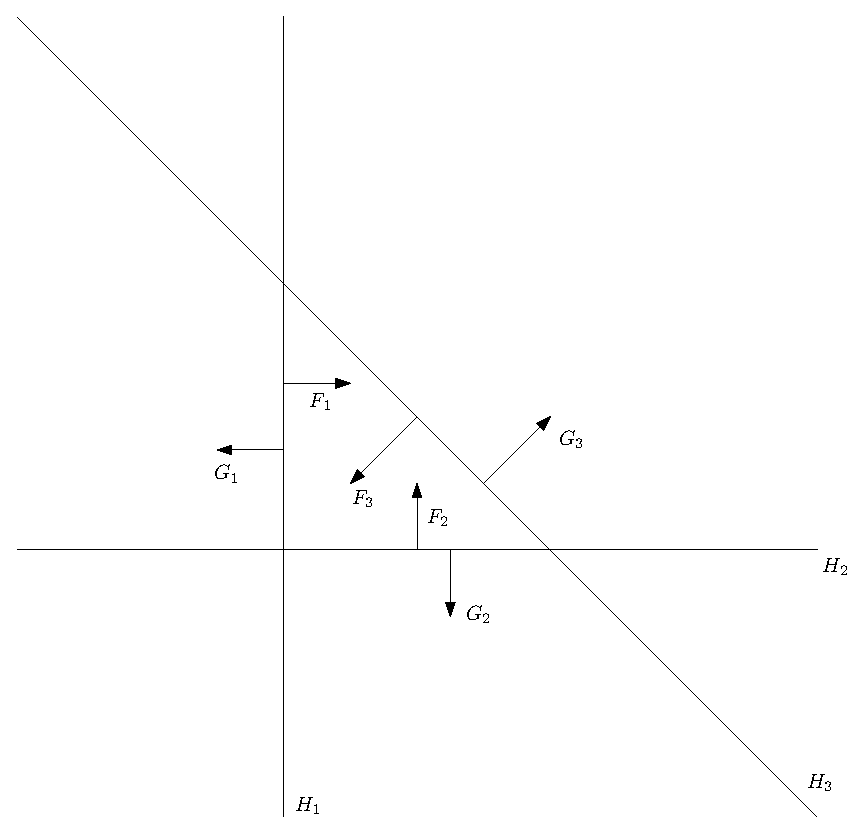
\includegraphics[width=10cm]{extended-core.eps}
\end{figure}

\begin{figure}[h!]
	\centering
	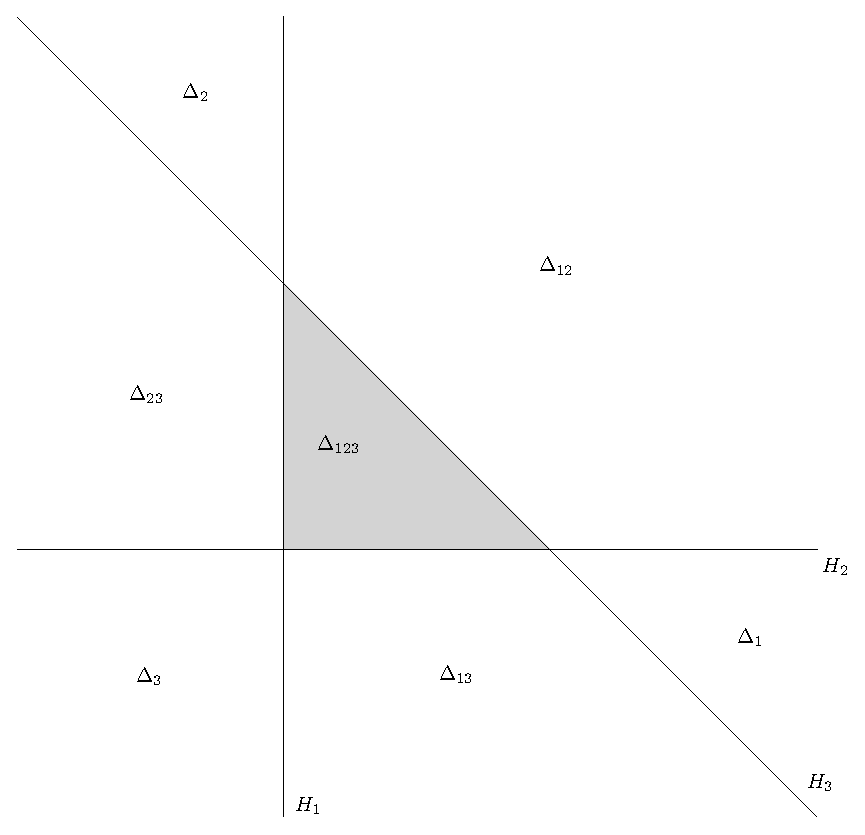
\includegraphics[width=10cm]{extended-core-polyhedra.eps}
\end{figure}

\newpage

Now $\CC^{\ast}$ does not act on $M$ as a subtorus of $T^{2}_{\CC}$, though it does when restricted to any single component of $\mc{E}_{A}$ of the extended core, with the action as a subtorus depending combinatorially on $A$.

For $[z,w] \in \mc{E}_{A}$ and $\tau \in \CC^{\ast}$,
\begin{equation*}
	\tau\cdot [z,w] = [z,\tau w] = [ \tau_{1}z_{1}, \tau_{2}z_{2}, \tau_{3}z_{3}, \tau_{1}^{-1}w_{1}, \tau_{2}^{-1}w_{2}, \tau_{3}^{-1}w_{3}],
\end{equation*}
where $\tau_{i} = \tau^{-1}$ if $i \in A$ and $\tau_{i} = 1$ if $i \not\in A$ (the subscripts are there emphasise that $\CC^{\ast}$ is acting as a subtorus of $T^{3}_{\CC}$). So the $\CC^{\ast}$-action on each $\mc{E}_{A}$ is determined via the inclusion $\tau \mapsto (\tau_{1}, \tau_{2},\tau_{3})$. For example, when $A = \{1,2\}$ the subtorus is $(\tau^{-1}, \tau^{-1}, 1) \subset T^{3}_{\CC}$.

Now consider the moment map for the $\CC^{\ast}$-action on $M$,
\begin{equation*}
	\begin{split}
	\Phi &:M \longrightarrow \RR_{\geq 0}\\
	\Phi[z,w] &= \frac{1}{2}\big(|w_{1}|^{2} + |w_{2}|^{2} + |w_{3}|^{2}\big).
	\end{split}
\end{equation*}

We will use it to symplectically cut the toric \HK manifold $M$ in order to compactify it as follows: consider the direct sum $M \times \CC$, where now $S^{1}$ acts on $M \times \CC$ as
$$
	e^{i\theta} \cdot \big( [z,w], \xi   \big) = \big( [z,e^{i\theta}], e^{i\theta}\xi\big),
$$
which is Hamiltonian with moment map
\begin{equation*}
\begin{split}
	\mu_{\text{cut}}:M \times \CC &\longrightarrow \RR_{\geq 0}, \\
		\mu_{\text{cut}}\big( [z,w], \xi  \big) &= \Phi[z,w] + \tfrac{1}{2}|\xi|^{2}.
\end{split}
\end{equation*}

Observe that $\mu_{\text{cut}}^{-1}(0) = \{ \big([z,0], 0\big) \in M \times \CC \} = X$, the toric \K manifold obtained from the Delzant polytope cut out by the hyperplane configuration, which in this example is $\CC\PP^{2}$.

Suppose now that $\e \in \RR_{\geq 0}$, then
\begin{equation*}
	\begin{split}
		\mu_{\text{cut}}^{-1}(\e) &= \big\{ ([z,w],\xi) \in M \times \CC \st \Phi[z,w] \leq \e \big\} \\
		&= \big\{ ([z,w], 0) \in M \times \{0\} \st \Phi[z,w] = \e \big\} \bigsqcup \big\{ ([z,w], \xi) \in M \times \CC \st \Phi[z,w] < \e \big\} \\
		&= \Phi^{-1}(\e) \bigsqcup \big\{ ([z,w], e^{i\phi}) \in M \times S^{1} \st \xi = e^{i\phi}\sqrt{2\e - \Phi[z,w]} \big\}\\
		&= \Sigma_{1} \sqcup \Sigma_{2}.
	\end{split}
\end{equation*}

Now since there exists a unique $S^{1}$-orbit through a $\xi \in \CC$ such that $\xi$ is actually real, with modulus $|\xi| = \sqrt{2\e - \Phi[z,w]}$, it follows that $\Sigma_{2}/S^{1}$ can be identified with $\big\{ [z,w] \in M \st \Phi[z,w] < \e \big\}$. Moreover $\Sigma_{1}/S^{1}$ is just the symplectic reduction $\Phi^{-1}(\e)/S^{1}$. Now these cut spaces still have the residual $S^{1}$-action from $\CC^{\ast}$ since it can be thought of as acting on $M \times \CC$ in the old sense on $M$ (rotating the fibres), and trivially on $\CC^{\ast}$, and this action commutes with the cutting action; in particular it remains Hamiltonian. Also note that the points of $M_{\text{cut}} = M_{\e > \Phi} \sqcup \Phi^{-1}(\e)/S^{1}$ which have a non-trivial stabiliser for the residual $S^{1}$-action occur when
$$
	\big( [z, e^{i\theta}w], \xi  \big) = \big( [z,e^{i\phi}w ], e^{i\phi}\xi \big)
$$
for some $e^{i\theta} \in S^{1} \setminus \{1\}$ and $e^{i\phi} \in S^{1}$, and that these new fixed points lie precisely in the level-set $\{ ([z,w], 0) \in M \times \CC \} = \Phi^{-1}(\e)$.

On each component $\mc{E}_{A}$ of the extended core, the cut introduces a half-space with normal determined by the Lie algebra generator for the $S^{1}$-action, as well as how $S^{1}$ acts on $\mc{E}_{A}$ as a subgroup of the torus $T^{3}$, e.g. on $\mc{E}_{12}$ where $S^{1}$ acts through the inclusion as $\tau \mapsto (\tau^{-1}, \tau^{-1}, 1)$, the normal vector is $-1\cdot u_{1} + -1\cdot u_{2} + 0\cdot u_{3} = (-1,-1)$, hence the polyhedron $\Delta_{12}$ is cut via the intersection
$$
	\Delta_{12} \cap \{ v\in \RR^{2} \st v \cdot (-1,-1) \geq \e \}.
$$

\begin{figure}[h]
	\centering
	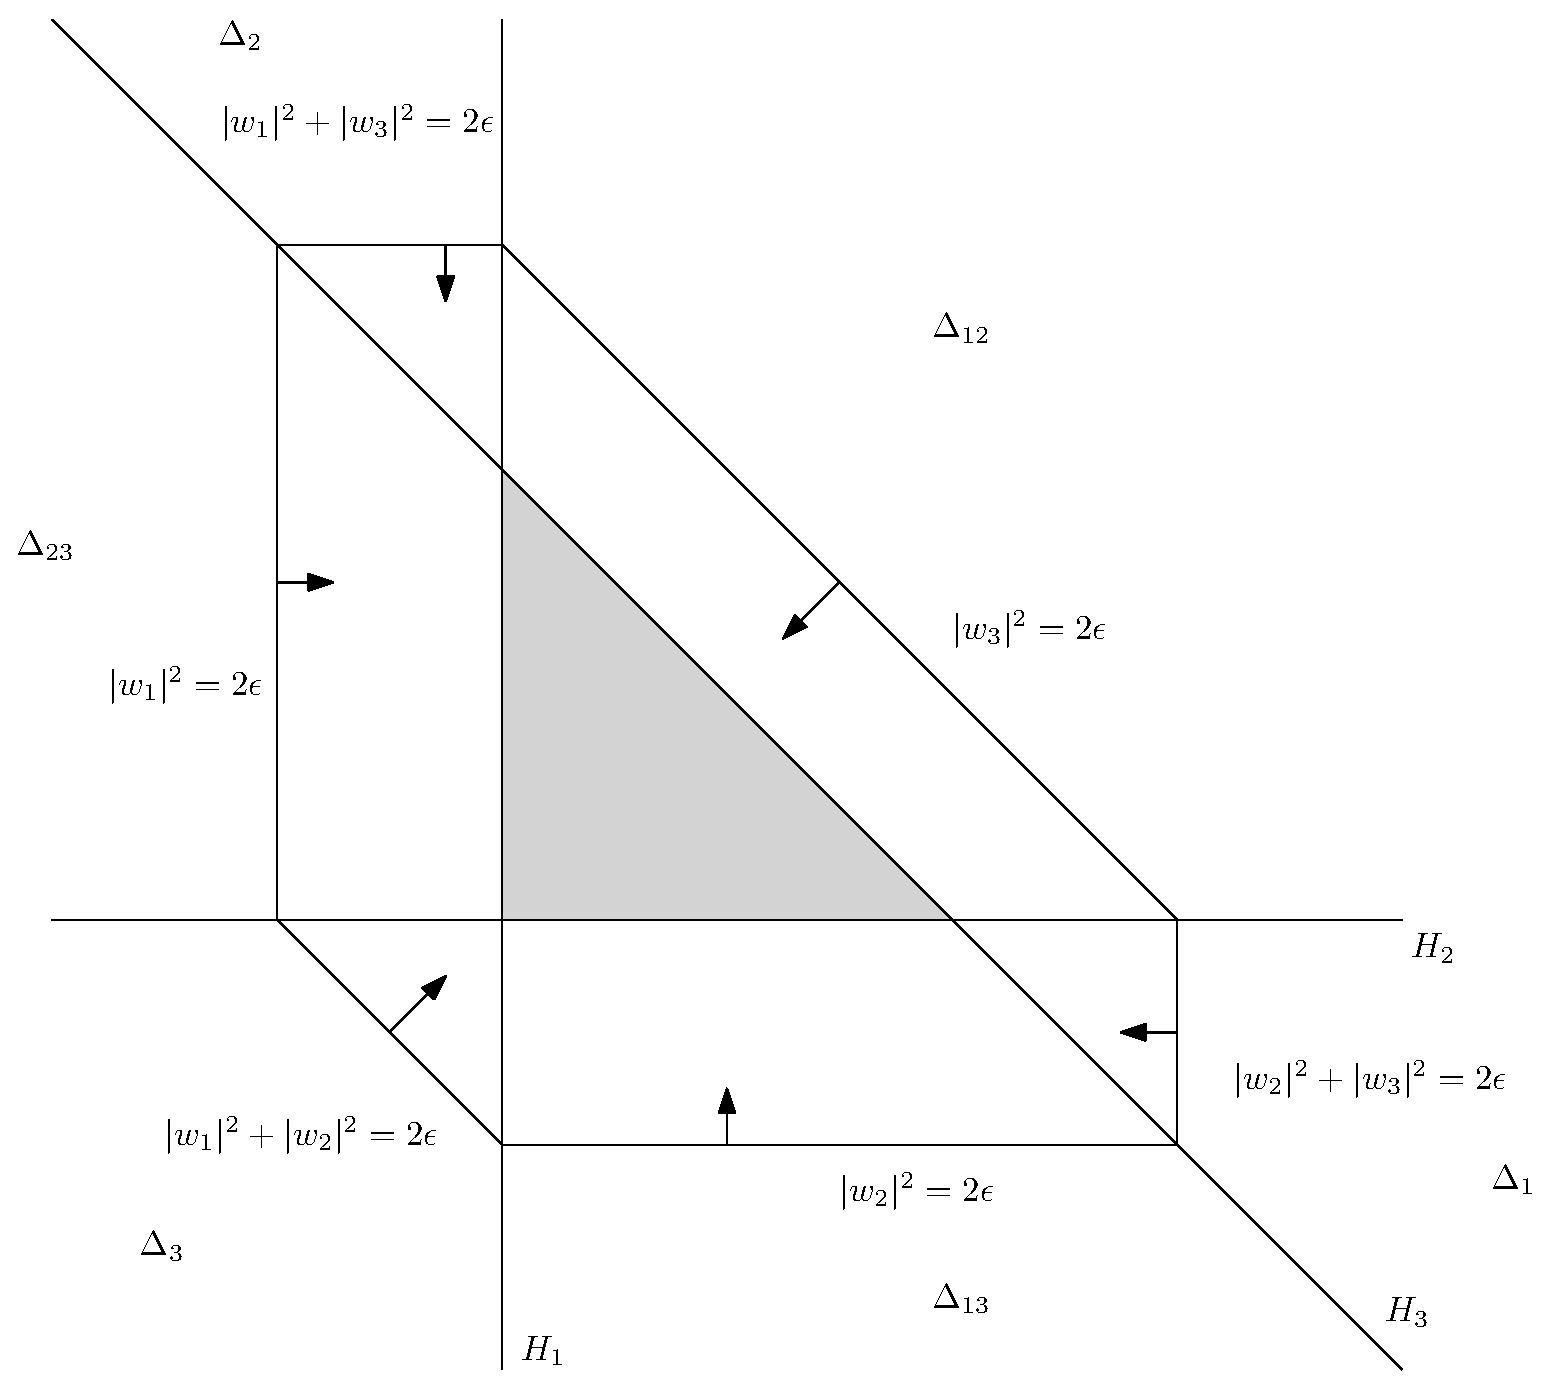
\includegraphics[width=12cm]{extended-core-cut.eps}\end{figure}

Let us look at how the cutting procedure affects each component $\mc{E}_{A}$ of the extended core individually.
\begin{equation*}
	\mc{E}_{A} \cap (\m_{\text{cut}}^{-1}(\e) / S^{1}) = 	\mc{E}_{A} \cap \bigg((\Sigma_{1} \sqcup \Sigma_{2})/S^{1}\bigg) \cong (\mc{E}_{A} \cap \Sigma_{2}) \sqcup \bigg( \mc{E}_{A} \cap  (\Phi^{-1}(\e)/S^{1})\bigg),
\end{equation*}
where
\begin{equation*}
	\mc{E}_{A} \cap (\Sigma_{2}/S^{1}) = \big\{ [z,w] \in \mc{E}_{A} \st \Phi[z,w] < \e \big\} = \bigg\{ [z,w] \in \mc{E}_{A} \st \tfrac{1}{2}\sum_{i \not\in A}|w_{i}|^{2} < \e \bigg\}
\end{equation*}
and
\begin{equation*}
	\begin{split}
		\mc{E}_{A} \cap  (\Phi^{-1}(\e)/S^{1}) &= \bigg\{ [z,w] \in \mc{E}_{A} \st \tfrac{1}{2}\sum_{i \not\in A}|w_{i}|^{2} = \e \bigg\}/S^{1} \\
		&= \bigg\{ [z,w] \in \mc{E}_{A} \st \tfrac{1}{2}\sum_{i \not\in A}|w_{i}|^{2} = \e,\text{ and } w_{i} \sim e^{i\theta}w_{i} \text{ for each } i \not\in A \bigg\} =: H_{A}
	\end{split}
\end{equation*}

We shall want to investigate the nature of the half-spaces $H_{A}$ that were introduced in the cutting procedure. First of all, recall that
\begin{equation*}
	\mc{E}_{A} = \bigg\{ [z_{1}, \ldots, z_{n}, w_{1}, \ldots, w_{n}] \in M \st w_{i} = 0 \text{ if } i \in A \text{ and } z_{i} = 0 \text{ if } i \not\in A \bigg\},
\end{equation*}
and also that the residual $S^{1}$-action on $M$ is given by
\begin{equation*}
	t\cdot [z,w] = [z_{1}, \ldots, z_{n}, tw_{1}, \ldots, tw_{n}].
\end{equation*}
Hence in introducing the symplectic cut, the quotient $\Phi^{-1}(\e)/S^{1}$ introduces additional stabiliser subgroups $N_{A}$ for each $\tilde{H}_{A}$, that act on $\tilde{H}_{A}$ through the inclusion into the original torus $T^{n}$.

Example: again when $A = \{1,2\}$, then
\begin{equation*}
	\mc{E}_{12} = \{ [z,w] \in M \st w_{1} = 0 = w_{2},\text{ and } z_{3} = 0 \} \cong \{ [z_{1}, z_{2}, 0; 0, 0, w_{3}] \in M \} = F_{1}\cap F_{2} \cap G_{3}.
\end{equation*}
Then the stabiliser subgroup $N_{12} \cong S^{1} \subset T^{3}$ for the residual $S^{1}$-action acting on the wall $\tilde{H}_{12}$ is $N_{12} \hookrightarrow T^{3}$, $t \mapsto (1,1,t)$, since $tw_{3} \sim w_{3}$ as a coordinate of $\mc{E}_{12} \cap (\Phi^{-1}(\e)/S^{1})$. Observe also that this action is equivalent to that of $t\cdot[z_{1}, z_{2}, w_{3}] = [t^{-1}z_{1}, t^{-1}z_{2}, w_{3}]$, when acting on $\mc{E}_{12}$.

After this discussion, set $N_{A} := (t_{i}, t_{i}, \ldots , t_{i} ) \subset T^{n}$, where $t_{i} = t^{-1}$ if $i \in A$ and $t_{i} = 1$ if $i \not\in A$; or equivalently $N_{A} = (t_{j}^{-1}, \ldots, t_{j}^{-1})$ where $t_{j} = t^{-1}$ if $j \not\in A$, and $t_{j} = 1$ if $j \in A$. Now set $\mf{n}_{A} := \Lie(N_{A})$, then $\mf{n}_{A}$ is generated by the vectors $\sum_{i \not\in A}u_{i} = -\sum_{i \in A}u_{i}$.

Example: $A = \{1,2\}$, then $N_{A} = (1,1,t)$ and $\mf{n}_{A} = (0,0,t)$, and also $\sum_{i \not\in A} u_{i} = u_{3} = (-1,-1)$. Thus
\begin{equation*}
	\tilde{H}_{A} = \{ x \in \RR^{2} \st \langle x, u_{3} \rangle + \e = 0 \} = \{ x \in \RR^{2} \st x + y = \e \}.
\end{equation*}

Since $N_{A}$ acts as a subtorus of $T^{3}$, this gives rise to a convenient way to evaluate the image of the moment map $\Phi |_{\mc{E}_{A}} : \mc{E}_{A} \rightarrow \RR$, namely
\begin{equation*}
	\Phi |_{\mc{E}_{A}}[z,w] = \bigg\langle \mu_{\RR}(z,w) , -\sum_{i \in A} u_{i} \bigg\rangle
\end{equation*}

The fixed point set of the residual $S^{1}$-action occurs when $\Phi|_{\mc{E}_{A}}$ is constant so that $d\Phi|_{\mc{E}_{A}} = 0$. Clearly this happens precisely on the locus $\Phi|_{\mc{E}_{A}}^{-1}(\e)$ (we ignore the case when $\e = 0$), and the $T^{d}$-stabiliser subgroup is generated by the Lie algebra spanned by the vectors $u_{k}$ that determine the $H_{i}$ and also $\tilde{H}_{A}$.




